%%%%%%%%%%%%%%%%%%%%%%%%%%%%%%%%%%%%%%%%%%%%%%%%%%%%%%%%%%%%%%%%%%%%%
%% This is a (brief) model paper using the achemso class
%% The document class accepts keyval options, which should include
%% the target journal and optionally the manuscript type.
%%%%%%%%%%%%%%%%%%%%%%%%%%%%%%%%%%%%%%%%%%%%%%%%%%%%%%%%%%%%%%%%%%%%%
\documentclass[journal=jacsat,manuscript=article]{achemso}

%%%%%%%%%%%%%%%%%%%%%%%%%%%%%%%%%%%%%%%%%%%%%%%%%%%%%%%%%%%%%%%%%%%%%
%% Place any additional packages needed here.  Only include packages
%% which are essential, to avoid problems later. Do NOT use any
%% packages which require e-TeX (for example etoolbox): the e-TeX
%% extensions are not currently available on the ACS conversion
%% servers.
%%%%%%%%%%%%%%%%%%%%%%%%%%%%%%%%%%%%%%%%%%%%%%%%%%%%%%%%%%%%%%%%%%%%%
\usepackage[version=3]{mhchem} % Formula subscripts using \ce{}
\usepackage[T1]{fontenc}       % Use modern font encodings

\usepackage{color}
\usepackage{xr}
\externaldocument{suppinfo}

%%%%%%%%%%%%%%%%%%%%%%%%%%%%%%%%%%%%%%%%%%%%%%%%%%%%%%%%%%%%%%%%%%%%%
%% If issues arise when submitting your manuscript, you may want to
%% un-comment the next line.  This provides information on the
%% version of every file you have used.
%%%%%%%%%%%%%%%%%%%%%%%%%%%%%%%%%%%%%%%%%%%%%%%%%%%%%%%%%%%%%%%%%%%%%
%%\listfiles

%%%%%%%%%%%%%%%%%%%%%%%%%%%%%%%%%%%%%%%%%%%%%%%%%%%%%%%%%%%%%%%%%%%%%
%% Place any additional macros here.  Please use \newcommand* where
%% possible, and avoid layout-changing macros (which are not used
%% when typesetting).
%%%%%%%%%%%%%%%%%%%%%%%%%%%%%%%%%%%%%%%%%%%%%%%%%%%%%%%%%%%%%%%%%%%%%
\newcommand*\mycommand[1]{\texttt{\emph{#1}}}

\newcommand{\cli}{Cl$^{-}$}
\newcommand{\ki}{K$^{+}$}

\newcommand{\nico}[1]{\textcolor{red}{#1}}
\newcommand{\kolya}[1]{\textcolor{blue}{#1}}
\newcommand{\denis}[1]{\textcolor{green}{#1}}

%%%%%%%%%%%%%%%%%%%%%%%%%%%%%%%%%%%%%%%%%%%%%%%%%%%%%%%%%%%%%%%%%%%%%
%% Meta-data block
%% ---------------
%% Each author should be given as a separate \author command.
%%
%% Corresponding authors should have an e-mail given after the author
%% name as an \email command. Phone and fax numbers can be given
%% using \phone and \fax, respectively; this information is optional.
%%
%% The affiliation of authors is given after the authors; each
%% \affiliation command applies to all preceding authors not already
%% assigned an affiliation.
%%
%% The affiliation takes an option argument for the short name.  This
%% will typically be something like "University of Somewhere".
%%
%% The \altaffiliation macro should be used for new address, etc.
%% On the other hand, \alsoaffiliation is used on a per author basis
%% when authors are associated with multiple institutions.
%%%%%%%%%%%%%%%%%%%%%%%%%%%%%%%%%%%%%%%%%%%%%%%%%%%%%%%%%%%%%%%%%%%%%
\author{Tsveta Miteva}
\affiliation{Sorbonne Universit\'{e}s, UPMC Univ Paris 06, UMR 7614, Laboratoire de Chimie Physique Mati\`{e}re et Rayonnement, F-75005 Paris, France}

\author{Nikolai Kryzhevoi}
\affiliation{Theoretische Chemie, Physikalisch-Chemisches Institut, Universit\"at Heidelberg, Im Neuenheimer Feld 229, D-69120 Heidelberg, Germany}

\author{Nicolas Sisourat}
\affiliation{Sorbonne Universit\'{e}s, UPMC Univ Paris 06, UMR 7614, Laboratoire de Chimie Physique Mati\`{e}re et Rayonnement, F-75005 Paris, France}

\author{{\color{red}Kirill ?}}
\affiliation{Theoretische Chemie, Physikalisch-Chemisches Institut, Universit\"at Heidelberg, Im Neuenheimer Feld 229, D-69120 Heidelberg, Germany}

\author{{\color{green}Nobuhiro Kosugi: acknowledgments?}}
\affiliation{Institute for Molecular Science, Myodaiji, Okazaki 444-8585, Japan}

\author{Ch. Nicolas}
\affiliation{Sorbonne Universit\'{e}s, UPMC Univ Paris 06, UMR 7614, Laboratoire de Chimie Physique Mati\`{e}re et Rayonnement, F-75005 Paris, France}

\author{Wandared Pokapanich}
\affiliation{Sorbonne Universit\'{e}s, UPMC Univ Paris 06, UMR 7614, Laboratoire de Chimie Physique Mati\`{e}re et Rayonnement, F-75005 Paris, France}

\author{Th. Saisopa}
\affiliation{Sorbonne Universit\'{e}s, UPMC Univ Paris 06, UMR 7614, Laboratoire de Chimie Physique Mati\`{e}re et Rayonnement, F-75005 Paris, France}

\author{P. Songsiriritthigul}
\affiliation{Sorbonne Universit\'{e}s, UPMC Univ Paris 06, UMR 7614, Laboratoire de Chimie Physique Mati\`{e}re et Rayonnement, F-75005 Paris, France}

\author{Y. Rattanachai}
\affiliation{Sorbonne Universit\'{e}s, UPMC Univ Paris 06, UMR 7614, Laboratoire de Chimie Physique Mati\`{e}re et Rayonnement, F-75005 Paris, France}

\author{Andreas Dreuw}
\affiliation{Interdisciplinary Center for Scientific Computing, Ruprecht-Karls University, Im Neuenheimer Feld 205A, D-69120 Heidelberg, Germany}

\author{Jan Wenzel}
\affiliation{Interdisciplinary Center for Scientific Computing, Ruprecht-Karls University, Im Neuenheimer Feld 205A, D-69120 Heidelberg, Germany}

\author{{\color{green}Matja\v{z} \v{Z}itnik: acknowledgments?}}
\affiliation{Sorbonne Universit\'{e}s, UPMC Univ Paris 06, UMR 7614, Laboratoire de Chimie Physique Mati\`{e}re et Rayonnement, F-75005 Paris, France}

\author{Ralph P\"{u}ttner}
\affiliation{Sorbonne Universit\'{e}s, UPMC Univ Paris 06, UMR 7614, Laboratoire de Chimie Physique Mati\`{e}re et Rayonnement, F-75005 Paris, France}

\author{J\'{e}r\^ome Palaudoux}
\affiliation{Sorbonne Universit\'{e}s, UPMC Univ Paris 06, UMR 7614, Laboratoire de Chimie Physique Mati\`{e}re et Rayonnement, F-75005 Paris, France}

\author{Gunnar \"{O}hrwall}
\affiliation{Sorbonne Universit\'{e}s, UPMC Univ Paris 06, UMR 7614, Laboratoire de Chimie Physique Mati\`{e}re et Rayonnement, F-75005 Paris, France}

\author{Jean Pascal Rueff}
\affiliation{Sorbonne Universit\'{e}s, UPMC Univ Paris 06, UMR 7614, Laboratoire de Chimie Physique Mati\`{e}re et Rayonnement, F-75005 Paris, France}
\affiliation{Synchrotron SOLEIL, l`Orme des Merisiers, Saint-Aubin, F-91192 Gif-sur-Yvette Cedex, France}

\author{Denis C\'{e}olin}
\email{denis.ceolin@synchrotron-soleil.fr}
\affiliation{Synchrotron SOLEIL, l`Orme des Merisiers, Saint-Aubin, F-91192 Gif-sur-Yvette Cedex, France}


%%%%%%%%%%%%%%%%%%%%%%%%%%%%%%%%%%%%%%%%%%%%%%%%%%%%%%%%%%%%%%%%%%%%%
%% The document title should be given as usual. Some journals require
%% a running title from the author: this should be supplied as an
%% optional argument to \title.
%%%%%%%%%%%%%%%%%%%%%%%%%%%%%%%%%%%%%%%%%%%%%%%%%%%%%%%%%%%%%%%%%%%%%
\title[]
  {The electronic structure of aqueous KCl revealed by X-ray absorption and Auger electron spectroscopy
\\  
  The all-seeing eye of Auger electron spectroscopy: a study on aqueous KCl}

%%%%%%%%%%%%%%%%%%%%%%%%%%%%%%%%%%%%%%%%%%%%%%%%%%%%%%%%%%%%%%%%%%%%%
%% Some journals require a list of abbreviations or keywords to be
%% supplied. These should be set up here, and will be printed after
%% the title and author information, if needed.
%%%%%%%%%%%%%%%%%%%%%%%%%%%%%%%%%%%%%%%%%%%%%%%%%%%%%%%%%%%%%%%%%%%%%
\abbreviations{AES,XAS}
\keywords{Solvated ions, Auger spectroscopy, X-ray absorption spectroscopy}

%%%%%%%%%%%%%%%%%%%%%%%%%%%%%%%%%%%%%%%%%%%%%%%%%%%%%%%%%%%%%%%%%%%%%
%% The manuscript does not need to include \maketitle, which is
%% executed automatically.
%%%%%%%%%%%%%%%%%%%%%%%%%%%%%%%%%%%%%%%%%%%%%%%%%%%%%%%%%%%%%%%%%%%%%
\begin{document}

%%%%%%%%%%%%%%%%%%%%%%%%%%%%%%%%%%%%%%%%%%%%%%%%%%%%%%%%%%%%%%%%%%%%%
%% The "tocentry" environment can be used to create an entry for the
%% graphical table of contents. It is given here as some journals
%% require that it is printed as part of the abstract page. It will
%% be automatically moved as appropriate.
%%%%%%%%%%%%%%%%%%%%%%%%%%%%%%%%%%%%%%%%%%%%%%%%%%%%%%%%%%%%%%%%%%%%%
\begin{tocentry}

\includegraphics[scale=0.82]{figures/graphical.png}
%Some journals require a graphical entry for the Table of Contents.
%This should be laid out ``print ready'' so that the sizing of the
%text is correct.
%
%Inside the \texttt{tocentry} environment, the font used is Helvetica
%8\,pt, as required by \emph{Journal of the American Chemical
%Society}.
%
%The surrounding frame is 9\,cm by 3.5\,cm, which is the maximum
%permitted for  \emph{Journal of the American Chemical Society}
%graphical table of content entries. The box will not resize if the
%content is too big: instead it will overflow the edge of the box.
%
%This box and the associated title will always be printed on a
%separate page at the end of the document.

\end{tocentry}

%%%%%%%%%%%%%%%%%%%%%%%%%%%%%%%%%%%%%%%%%%%%%%%%%%%%%%%%%%%%%%%%%%%%%
%% The abstract environment will automatically gobble the contents
%% if an abstract is not used by the target journal.
%%%%%%%%%%%%%%%%%%%%%%%%%%%%%%%%%%%%%%%%%%%%%%%%%%%%%%%%%%%%%%%%%%%%%
\begin{abstract}
 \nico{X-ray absorption and Auger electron spectroscopies are powerful tools to probe the electronic structure and immediate surroundings of ions in a solution. In this work we use a combination of these spectroscopies to study the electronic structure and decay of aqueous KCl at the K-edges of \ki~and \cli.}
%Auger electron spectroscopy is a powerful tool to probe the electronic structure and immediate surroundings of ions in a solution. In this work we use a combination of x-ray absorption and Auger electron spectroscopies to study the electronic structure and decay of aqueous KCl at the K-edges of \ki~and \cli. 
Although the two ions are isoelectronic, their Auger electron spectra as a function of the photon energy exhibit notably different features. To explain these differences, we carried out {\it ab initio} calculations of both the core excited states and the final Auger states of \ki, \cli~and their microsolvated clusters. Our calculations show that the energy order of the 3d and 4p orbitals is inverted in \ki~with respect to \cli. 
%
%The reverse orbital order in the two ions not only influences the x-ray absorption spectra, but also impacts the course of the subsequent resonant Auger processes.
%
The reverse orbital order in the two ions is reflected in both the ordering of the core excited states and in the final states populated in the resonant Auger decay. \nico{Furthermore}, the energetic proximity of the 3d and 4p virtual states in \nico{the }\ki~\nico{bare ion} leads to their mixing in the presence of the solvent, and to the population of the dipole forbidden 1s$\,\rightarrow\,$3d state upon K-shell excitation in an aqueous solution. The resonant Auger decay of this state results in a separate feature in the Auger electron spectrum of \ki~which is absent in the spectrum of \cli.
\end{abstract}

%%%%%%%%%%%%%%%%%%%%%%%%%%%%%%%%%%%%%%%%%%%%%%%%%%%%%%%%%%%%%%%%%%%%%
%% Start the main part of the manuscript here.
%%%%%%%%%%%%%%%%%%%%%%%%%%%%%%%%%%%%%%%%%%%%%%%%%%%%%%%%%%%%%%%%%%%%%
\section{Introduction}
% Paragraph 1: introduction to AES and XAS/AES and what are they needed for. if possible, find a combination of the two to explan that this is a more powerful tool to study the electronic structure


X-ray absorption and Auger electron spectroscopies are powerful tools to study the electronic structure and the nearest environment of atoms and molecules in gas, liquid and solid phase. Understanding how atoms or molecules respond to irradiation with x-rays gives insight into the structure of solutions \citep{Pokapanich09:7264}, and the mechanism of radiation damage \citep{ONeill02:329,Carugo05:213,Stumpf16:237}. Upon absorption of an x-ray photon, core excited or core ionized states of a specific atom are populated depending on the photon energy. The relaxation of these highly energetic states involves an ultrafast cascade of intraatomic processes, such as radiative and Auger decay. Furthermore, if the initially excited or ionized species is embedded in an environment, interatomic processes such as interatomic Coulombic decay (ICD) and related processes \citep{Pokapanich09:7264,Pokapanich11:13430,Stumpf16:237,unger17:708} are possible.


The course of a decay cascade depends on the character of the initially populated states. This has been well understood in atoms and molecules in gas phase (REFS) \citep{stoychev08:074307,Demekhin08:043421,Demekhin09:104303,Ouchi11:053415,Miteva14:164303,Miteva14:064307}. In the case of a core ionized state, the Auger decay process, designated as normal Auger decay (see Fig.\ \ref{fg:auger}), leads to the population of doubly ionized final states localized on the initially ionized unit \citep{stoychev08:074307,Demekhin08:043421,Demekhin09:104303,Ouchi11:053415}. \nico{Auger processes in rare gas clusters have been also investigated (refs).} The normal Auger decay process in clusters proceeds similarly to that in atoms or molecules. \nico{However,} In the case of a core excited state, the resonant Auger process competes with the process of delocalization of the excited electron in clusters \citep{Bjorneholm95:3017}. If the initially core excited electron delocalizes within the lifetime of the core hole, then normal instead of resonant Auger decay is observed \citep{Bjorneholm95:3017}. 


In a solution, the electronic decay cascades initiated by x-ray photoabsorption are different compared to those in rare gas clusters due to the shorter distances and stronger interatomic interactions. In particular, the solvent molecules have two effects -- first, they strongly affect the excited \citep{miteva16:16671} or ionized states of the ion and second, they can participate in the decay processes, leading to the population of delocalized final states, and thus ionizing the surrounding environment \citep{Pokapanich09:7264,Pokapanich11:13430,Stumpf16:237}. 
\nico{Moreover, the process of delocalization of the initially excited electron also occurs in aqueous solutions \citep{Nordlund07:217406,Ottosson11:13489}.}
%Moreover, the process of delocalization of the initially excited electron is not specific to rare gas clusters, but it also occurs in aqueous solutions \citep{Nordlund07:217406,Ottosson11:13489}. 
In the case of pure water, the rate of delocalization of the O1s excited electron takes place on a femtosecond to sub-femtosecond time scale depending on the photon energy, thus being commensurate with the lifetime of the O1s core hole which is 6\,fs \citep{Nordlund07:217406}. The O K-edge is located in the soft x-ray range of photon energies. Going higher in photon energy, in the hard x-ray regime, the lifetimes of the core ionized or core excited states become even shorter, on the order of 1\,fs (REF). And thus, it is even more imperative to reveal whether the delocalization of the core excited electron occurs within the lifetime of the core hole.


The aim of this work is to elucidate the nature of the states populated upon x-ray irradiation of solvated ions in the hard x-ray regime, and furthermore, to understand whether the process of delocalization influences the resonant Auger decay. To this end, we used Auger electron spectroscopy together with x-ray absorption spectroscopy in the hard x-ray regime to study aqueous potassium chloride at the K-edges of both \ki~and \cli. In particular, we demonstrate experimentally that at photon energies below the K-edges of the two ions, localized core excited states are populated. These states undergo resonant Auger decay within less than 1\,fs. In both ions, there is a competition between resonant Auger decay and delocalization of the excited electron. Using the core-hole clock method (REFS), we show that in \ki~delocalization at the pre-edge is weak, whereas in the case of \cli, due to the energetic proximity of the core excited state to the K-edge, the rate of delocalization is of the same order as that of the resonant Auger process. Moreover, we observe that although the \ki~and \cli~ions are isoelectronic, they have different fingerprints in the resonant Auger spectra. With the aid of high-level {\it ab initio} calculations of the initial and final states of the resonant Auger process of both the bare ions and their microsolvated clusters, we demonstrate that these differences are a result of the different electronic structure of the two ions, thus confirming that the XAS/AES technique is a sensitive probe of the electronic structure of solutions.


\begin{figure}
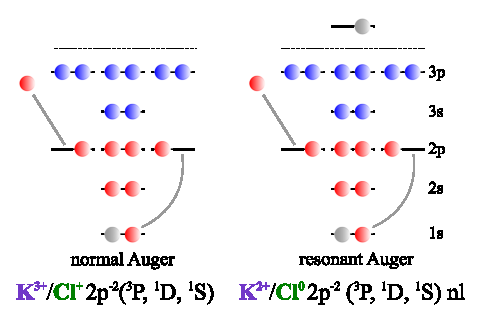
\includegraphics{figures/auger_process.eps}
\caption{Schematic representation of the normal and resonant Auger processes.}
\label{fg:auger}
\end{figure}

\section{Methods} \label{sec:methods}
\subsection{Experimental}
% Denis, please have a look at the experimental part and see if all the references have been correctly included

For the present experiment we used the newly operational microjet setup that was specifically designed for the HAXPES station of the GALAXIES beamline, in collaboration with the Microliquids Company. Details of the beamline are given in the reference [JPR] and details on the electron spectrometer are given in the reference \citep{ceolin15:022502,ceolin13:188}. Due to the limited amount of space available if front of the analyzer lens and due to the limited number of ports available on the main vacuum chamber, the challenge was to arrange all the elements composing the microjet setup in a very compact manner. A differentially-pumped tube in which the microjet assembly is inserted, is installed in front of the spectrometer lens and can be moved independently from the main vacuum chamber by means of a three axes motorized manipulator. Two holes of 2 mm diameter allow the photons to go in and out of the tube, and a third one, on which is mounted a skimmer having a 500$\mu$m diameter hole, allows the electrons created at the interaction point to go in the direction of the spectrometer lens. To ensure a proper vacuum in the differentially pumped tube, a 5-way cross is connected to it and holds a 1200 l/s turbo pump, a liquid nitrogen trap, a vacuum gage and the liquid/electrical feedthroughs. A rail, fixed at the bottom of the tube, is used to slides precisely an insert on which the different elements necessary for the injection, control, collection and visualization of the liquid are mounted.


The head of this insert is mostly composed by: a glass capillary fixed by a dedicated peek-piece, a catcher in CuBe with a 300$\mu$m hole, a piezo motors stage allowing a precise control of these last two parts, and a camera. The catcher is placed at a distance of about 5mm from the capillary and is permanently pumped in order to extract the liquid from the vacuum chamber. For the present experiment, a 0.5M KCl aqueous solution is injected in a capillary having a 30$\mu$m diameter, by a HPLC pump with a constant flux of 1.6 ml/min. The catcher temperature is controlled so that the liquid does not freeze before its extraction. Considering that the photon propagation axis, the spectrometer lens axis and the liquid microjet form an orthogonal trihedron, the piezo motorization allows moving the liquid microjet along the photon propagation and the lens axes during the experiment if necessary. The catcher can be moved by the piezo motors along the photon propagation axis only. A simple camera is used to control the liquid jet positioning as compared with the catcher hole. The alignment of the full head (particularly capillary plus catcher) as compared with the X-ray beam is performed by moving the whole system using the 3-axes motorized manipulator. The alignment of the setup is performed by measuring the O1s XPS peak intensity of a simple salt aqueous solution, and by optimizing the liquid phase vs gas phase ratio. The pressure in the main chamber was kept below the 10$^{-5}$ mbar range whereas it was kept at about 10$^{-4}$ mbar in the differentially pumped tube when the HPLC pump was ON. Our equipment is an updated version of the equipment used in the references [3-5]. The aqueous potassium chloride solution was prepared by mixing >99\% KCl salt with deionized water. Filtering and degazing procedures were systematically performed before injecting the solution into the microjet by the HPLC pump. \denis{The spectrometer resolution of about 0.6 eV was achieved with the 500 eV pass energy and 0.5 mm slits. The photon energy resolution achieved at 2.8 keV and 3.6 keV was about 0.3 eV and 0.4 eV respectively}. 


\subsection{{\bf{\it Ab initio}} calculations}

The X-ray absorption spectra of the microsolvated clusters of potassium and chlorine were computed at the ground state equilibrium geometries of K$^+$(H$_2$O)$_6$ and \cli(H$_2$O)$_6$, which can be considered as representatives of the complete first solvation shell of the two ions \citep{Ohtaki93:1157,soper06:180,ma14:1006}. The two structures were optimized at the DFT level of theory using the B3LYP functional and the 6-311++G(2d,2p) basis set \citep{Krishnan80:650,Blaudeau97:5016}. A frequency analysis was carried out in order to confirm that the obtained geometries are minima on the respective potential energy surfaces. The geometry optimization and frequency analysis were performed with the Gaussian 09 package \citep{g09}. In the case of K$^{+}$(H$_2$O)$_6$ the ground state geometry was obtained by constrained geometry optimization starting with the equilibrium geometry \citep{lee99:3995} belonging to the D$_3$ point group and increasing the angle $\theta$ between the K-O bond and the $C_3$ axis to 55$^{\circ}$. This angle was chosen to be around the maximum in the O-K-O angular distribution obtained from quantum mechanics / molecular mechanics dynamical simulations in Ref.\ \citep{ma14:1006}. {\color{red} the maximum is at 70$^{\circ}$, in our calculation the angle is 90$^{\circ}$} The optimized K-O and Cl-O distances are 2.842~\AA~and 3.333~\AA, respectively, which is in good agreement with other theoretical and experimental works \citep{ge13:13169,gora00:7,Ohtaki93:1157,soper06:180,ma14:1006}. The ground state equilibrium structures are presented in Fig.\ \ref{fg:xas_kcl}. In both cases, they belong D$_3$ point group \citep{rao08:12944,ge13:13169}. 


The energies and transition moments of the core excited states of the microsolvated clusters were computed with the algebraic diagrammatic construction method for the polarization propagator \citep{sch82:2395} within the core-valence separation approximation \citep{bar85:867,ced80:206,ced81:1038} (CVS-ADC(2)x) as implemented in the Q-Chem package \citep{Wenzel14:1900,Wenzel14:4583,Wormit14:774,QChem2015}. In the case of \cli, the 6-311++G(3df,3pd) basis set \citep{Krishnan80:650,McLean80:5639} (excluding the f functions) was used on all atoms, whereas in the case of \ki, we used the 6-311+G(2d,p) basis set \citep{Krishnan80:650,Blaudeau97:5016} on all atoms, and an additional set of 2s, 2p and 2d diffuse functions was added on K. In our calculations, the core space comprises the 1s orbital of K$^{+}$ or \cli, whereas the remaining occupied orbitals are included in the valence space. For the calculations of the XAS spectra we used the C$_2$ point group in the case of K$^{+}$(H$_2$O)$_6$ and \cli(H$_2$O)$_6$. To account for the lifetime broadening due to the Auger decay of the core excited states, we convolved the theoretical spectra with a Lorentzian of FWHM 0.74\,eV and 0.62\,eV in the case of \ki~and \cli, respectively \citep{Krause79:329}. We analyzed the core excited states by expanding the singly occupied natural orbitals (SONOs) $\psi_{i}$ of the microsolvated clusters in the basis of SONOs of the bare K$^{+}$ or \cli~ion $\chi_{nl}$
%
\begin{equation}\label{eq:sono_proj}
\psi_{i} = \sum_{nl} a^{i}_{nl} \chi_{nl}
\end{equation}
%
where $n$ and $l$ stand for the principal and orbital quantum numbers as described in Ref.\ \citep{miteva16:16671}. The expansion coefficients $a^{i}_{nl}$ show the degree of delocalization of the excited electron and the mixing of the core excited states in the crystal field created by the surrounding water molecules (see Fig.\ \ref{fg:xas_kcl}).


The final states following KLL resonant Auger decay of K$^{+}$ and \cli~were computed at the Configuration Interaction Singles (CIS) level using the Graphical Unitary Group Approach (GUGA) as implemented in the GAMESS-US package \citep{GUGA_PhysScr_21,GUGA_JCP_70,GUS}. In order to account for the relaxation effects upon core ionization, we used a restricted open-shell Hartree-Fock reference wave function with a hole in the 2s orbital of both \ki~and \cli.  We used the 6-311++G(2d,2p) basis set \citep{Blaudeau97:5016} augmented with 2s, 2p, 2d diffuse functions on \ki, and the cc-pVTZ basis set augmented with 6s, 6p, 6d diffuse KBJ functions \citep{Kaufmann89:2223} on \cli. The active space comprises the 2s and 2p orbitals of K/Cl with occupancy fixed to 6 and all virtual orbitals with occupancy fixed to 1. The remaining doubly occupied orbitals were frozen in the calculation. \citep{mosnier16:061401}

\section{Results}\label{sec:results}

% Question to Denis: how exactly do you extract the IP from the XPS spectrum?
%{\color{blue}
%THESE RESULTS ARE ALREADY reported in the other paper, so we don't need them here, do we?
%
%The ionization potentials (IP) of Cl$^{-}$1s and K$^{+}$1s were measured by XPS at $h\nu = 5$\,keV, far enough from the threshold to minimize PCI effects, and calibrated on the O1s (liquid) binding energy taken at 538.1\,eV \citep{winter06:1176}. We found the value of 2825.4\,eV for the ionization potential of Cl$^{-}$ 1s (Fig.\ \ref{fg:2dmap_cl}) and 3611.9\,eV for K$^{+}$ 1s (Fig.\ \ref{fg:2dmap_k}). The full width half-maximum of these main lines was extracted and their Lorentzian contribution was measured at 0.72\,eV for K$^{+}$1s(aq) and 0.62\,eV for Cl$^{-}$1s(aq). This result agrees well with the corresponding theoretical values of 0.74\,eV and 0.64\,eV for bare potassium and chloride taken from Ref.\ \citep{Krause79:329}. In the X-ray energy region of the ionization potential of aqueous Cl$^{-}$, the photon bandwidth provided by the double crystal monochromator is about {\color{red}0.4\,eV}, whereas in the region of the ionization potential of aqueous K$^{+}$, the photon bandwidth is about {\color{red}0.5\,eV}.}


In this section we discuss the experimental results presented as 2D maps showing the dependence of the kinetic energy of the Auger electrons on the photon energy scanned across the K-edges of the aqueous potassium (Fig.\ \ref{fg:2dmap_k}) and chloride ions (Fig.\ \ref{fg:2dmap_cl}), 3611.9\,eV and 2825.4\,eV, respectively \citep{ceolin17}. The range of electron kinetic energies of the corresponding relaxation channels is larger than 2\,keV, which corresponds to inelastic mean free paths of about 50~\AA~or more in liquid water \citep{emfiet09:45}. The energies thus allow us to probe the bulk of the sample and, moreover, they ensure that the electrons escape the liquid with a sufficient count rate.


\begin{figure}%[h!]
\centering
\includegraphics[scale=0.55]{figures/2Dmap_K1s_XAS.pdf}
\caption{2D map showing the kinetic energy of the electrons emitted in $K L_{2,3}L_{2,3}$ Auger decay vs the photon energy in the vicinity of the K-edge of aqueous K$^{+}$. The black curve on the left represents the experimental partial electron yield spectrum of K$^{+}$ obtained after integrating over the kinetic energies of the Auger electrons.\\
{\color{red}\bf @Denis, can you please add the letters B and C on the 2D map, and also make the 2D maps of \ki~and \cli~the same size and use the same font size?}}
\label{fg:2dmap_k}
\end{figure}


\begin{figure}%[h]
\centering
\includegraphics[scale=0.65]{figures/2Dmap_Cl1s_XAS.pdf}
\caption{2D map showing the kinetic energy of the electrons emitted in $K L_{2,3}L_{2,3}$ Auger decay vs the photon energy in the vicinity of the K-edge of aqueous Cl$^{-}$. The black curve on the left represents the experimental partial electron yield spectrum of Cl$^{-}$ obtained after integrating over the kinetic energies of the Auger electrons.}
\label{fg:2dmap_cl}
\end{figure}


\subsection{Normal Auger decay}\label{ssec:na}

Let us first consider the vertical lines at photon energies $h\nu = 3617$\,eV {\color{red}(spectrometer resolution)} on Fig.\ \ref{fg:2dmap_k} and $h\nu = 2830$\,eV {\color{red}(spectrometer resolution)} on Fig.\ \ref{fg:2dmap_cl}, respectively. They originate from KL$_{2,3}$L$_{2,3}$ Auger decay following the core ionization of K$^+$ and Cl$^-$, which leads to the population of $^3P$, $^1D$, and $^1S$ $2p^{-2}$ final states
%
\begin{align*}
h\nu + \text{K}_\text{aq}^{+} \rightarrow \text{K}_\text{aq}^{++}(1s^{-1}) + e^{-}_{\text{ph}}
			 \rightarrow \text{K}_\text{aq}^{3+} (2p^{-2}\ \ ^3P,\ ^1D,\ ^1S) + e^{-}_{\text{ph}} + e^{-}_{\text{Auger}} \\
h\nu + \text{Cl}_\text{aq}^{-} \rightarrow \text{Cl}_\text{aq}^{0}(1s^{-1}) + e^{-}_{\text{ph}}
			 \rightarrow \text{Cl}_\text{aq}^{+} (2p^{-2}\ \ ^3P,\ ^1D,\ ^1S) + e^{-}_{\text{ph}} + e^{-}_{\text{Auger}} 
\end{align*}
%
In the case of Cl$^{-}_{\text{aq}}$, the lines corresponding to the Cl$^{+}$ (2p$^{-2}$) $^1$S, $^1$D and $^3$P states are located at 2373.2\,eV, 2382.1\,eV and $\sim$2390\,eV kinetic energy. The position of the $^{3}$P line is determined approximately as the line is obscured by the dispersive feature with a maximum at 2825.2\,eV photon energy and 2383.5\,eV kinetic energy (see Fig.\ \ref{fg:2dmap_cl}). For K$^{+}_{\text{aq}}$ the maxima of the $^1$S and $^1$D KL$_{2,3}$L$_{2,3}$ Auger lines are located at 2958\,eV and 2968.4\,eV, respectively (see Fig.\ \ref{fg:2dmap_k}). The intensity of the $^3$P line is too weak and it cannot be clearly distinguished from the high-kinetic energy tail of the $^1$D line and from one of the dispersive lines with a maximum at 2969.5\,eV.


The KL$_{2,3}$L$_{2,3}$ Auger lines are not supposed to disperse with the photon energy except close to threshold due to the interaction between the photoelectron and Auger electron, i.e.\ the so-called post-collision interaction (PCI). As a result of this interaction, first, the peaks in the Auger spectrum become asymmetric with a shoulder at high kinetic energies, and second, they are shifted to higher kinetic energies close to threshold \citep{russek86:911,guillemin15:012503}. Consequently, one can attribute the high kinetic energy shoulder of the $^1$D and $^1$S peaks on Figs.\ \ref{fg:2dmap_k} and \ref{fg:2dmap_cl} as resulting from PCI effect. In order to minimize this effect we recorded the KLL Auger spectrum of both Cl$^{-}_{\text{aq}}$ and K$^{+}_{\text{aq}}$ at higher photon energies, $h\nu = 5$\,keV. The maxima of the $^3$P, $^1$D and $^1$S states were found at 2389\,eV, 2381.1\,eV and 2372.3\,eV for Cl$^{-}_{\text{aq}}$, and 2976.3\,eV, 2967.4\,eV and 2957\,eV kinetic energy for K$^{+}_{\text{aq}}$, respectively. The lines observed at a photon energy far from threshold and close to it appear to be shifted by $\sim$1\,eV. The magnitude of the shift is the same for both ions, thus, we can conclude that it does not depend on the initial charge of the ion. The observed PCI shift of 1\,eV is larger than in the case of the isoelectronic Ar, where its value is $\sim$0.5\,eV at a photon energy of 10 \,eV above threshold \citep{guillemin15:012503}. The shift in the energies of the photo- and Auger electrons is proportional to the change in the ionic field during the Auger process. In a solution, both the initial and the final Auger states will be stabilized as a result {\color{red}of ion-dipole interaction with the surrounding polarizable medium (?)}. The magnitude of this effect increases with the ionic charge. Thus, one can expect a larger change in the ionic field in an aqueous solution compared to that in a van der Waals cluster, which can, therefore, account for the large PCI shift of the Auger lines in a solution.


The normal Auger $^1$D main line of K$^{+}$ differs from that of Cl$^{-}$ by the presence of a large shoulder on the low kinetic energy side at about 2965\,eV kinetic energy. This shoulder is a result of a charge transfer process to the solvent molecules which will be the subject of a separate article \citep{ceolin17}.


\subsection{Resonant Auger decay} \label{ssec:ra}
Next, we discuss the dispersive features in the spectra of aqueous \ki~and \cli~originating from the resonant Auger decay of the core excited states below threshold. In order to get a better understanding of these features, we will first consider the Auger spectrum of the isoelectronic Ar presented in Refs.\ \citep{ceolin15:022502,guillemin15:012503}. 


First, from the 2D map of Ar one can extract information about the nature of the core excited states below threshold. The pre-edge structure in the XAS spectrum of Ar consists of the 1s$\,\rightarrow\,$4p and 1s$\,\rightarrow\,$5p excitations. Higher core excited states cannot be identified in the XAS spectrum due to their lifetime broadening and proximity to the ionization threshold. The same excitations were observed in the XAS spectrum of bare \ki~ions \citep{hertlein06:062715}. Again, the identification of 1s$\,\rightarrow\,$np states with n$> 5$ was not possible in the case of \ki.


Second, the 2D map of Ar one can extract information about the positions of the final Auger states - both in the normal and resonant Auger processes. In the case of Ar, the Ar $1s \rightarrow 4p$ and $1s \rightarrow 5p$ core excited states undergo both pure spectator and shake-up resonant Auger decay leading to the population of Ar$^{2+}(2p^{-2} np)$ ($n = 4 - 7$) final states. As a result, apart from the main Ar$^{2+}(2p^{-2})$ $^1$D and $^1$S lines which result from normal Auger decay, additional islands are observed. For example, the $1s \rightarrow 4p$ core excited state undergoes both pure spectator and shake-up resonant Auger decay. The former results in an island shifted with respect to the main $^1D$ line by $\sim$4-5\,eV kinetic energy, whereas the fingerprint of the shake-up process is a feature appearing at the same kinetic energy as the  main $^1D$ line. Moreover, the intensities of the observed shake-up features are lower compared to those of the pure spectator Auger decay. In aqueous solutions, one can expect the 2D map to be fairly different as both the initial core excited states and the final Auger states will be influenced by the presence of the solvent. 


\underline{Chloride ion Cl$^{-}$}

% 3: discussion of the dispersive lines; they are not observed in the XAS spectrum, because they overlap with the ... but they are visible on the 2D map; they result from resonant Auger decay of the 1s --> np transition in Cl-

Let us consider the features on Fig.\ \ref{fg:2dmap_cl} designated by dashed lines. Since they disperse with photon energy, they originate from Auger decay of a resonant K-shell excitation. From the 2D map we can determine the position of this core excitation at 2825.2\,eV. It is located only 0.2\,eV below the $1s$ ionization potential of Cl$^{-}_{\text{aq}}$, whose natural lifetime broadening is 0.62\,eV \citep{Krause79:329}. This state is therefore not visible in the XAS spectrum presented to the left on Fig.\ \ref{fg:2dmap_cl}, but only in a combined XAS and AES experiment. The excitation energy of 2825.2\,eV agrees very well with the position of the Cl$^{-}$ $1s \rightarrow 4p$ excitation determined by Cl K-edge XAS experiments in MgCl$_2$.6H$_2$O and of SrCl$_2$/SrCl$_2$.6H$_2$O \citep{sugiura82:681} and XXX \citep{rompel97:4465}. Contrary to the case of Ar \citep{ceolin15:022502}, with which Cl$^{-}$ is isoelectronic, a separate shake-up feature is not observed in this case.


{\color{red}
However, for atomic chloride, the description of the excited states in terms of Rydberg series is possible because the promoted electron sees an ionic core of a +1 charge. In the case of chlorine, the situation is different since the charge seen by the 1s promoted electron is null and thus using a Rydberg series description is not appropriate. More generally, it is known that isolated halide ions have no bound excited states (Berry, R. S.; Reimann, C. W.; Spokes, G. N. J. Chem. Phys. (1962), 37, 2278, Wen-Shyan Sheu and Peter J. Rossky, J. Phys. Chem. (1996), 100, 1295). However, when surrounded by water molecules, delocalized states as CTTS states have been highlighted by various MD simulations (Staib, A.; Borgis, D., J. Chem. Phys. 104, (1996), 9027 and J. Chem. Phys. 103, (1995) 2642) and experimental methods, including resonant Auger spectroscopy performed in the vicinity of the Cl-2p ionization threshold, as demonstrated by Winter et al. (JACS, 130 (2008) 7130). In the present case, we excite a s-type symmetry orbital so we expect to populate mostly p-type orbital(s). Staib, A.; Borgis, D., (J. Chem. Phys. 104, (1996), 9027 and J. Chem. Phys. 103, (1995) 2642) have calculated density of states for Cl-(aq) and highlighted a dense manifold of p-symmetry states followed by s/d symmetry states in an energy region just below the electron photo detachment threshold value, i.e., from about -1 eV to 0 eV. In our case, the 1s-1-first unoccupied state maximum is at about 0.2eV below threshold, but the corresponding core-excited state has a natural broadening of about 0.6 eV FWHM, meaning thus that the core-excited states overlap (SORRY, here again I need to add arguments).

}


\underline{Potassium ion K$^{+}$}

The calibrated (?) 2D map corresponding to the relaxation of solvated potassium ion excited in the vicinity of its K-edge is presented on Fig.\ \ref{fg:2dmap_k}. Two dispersive lines are observed in Fig.\ \ref{fg:2dmap_k}; they have maxima at $h\nu = $3611.2 \,eV and 2969.2 \,eV kinetic energy, and $h\nu = $3611.6\,eV and 2978.1\,eV kinetic energy, respectively. The first dispersive feature appears as an island, separated by approximately 8.3\,eV kinetic energy from the second dispersive feature, which on its turn is close to the $^1$D main line. Unlike in the case Cl$^{-}$ the dispersive feature close to the $^1$S main line is not found in K$^{+}$ due to presence of a strong {\color{red}BACKGROUND}.

\section{Conclusion}\label{sec:concl}

Using a combination of x-ray absorption and Auger electron spectroscopy, in this work we study the electronic structure of aqueous solution of KCl at the K-edges of both K and Cl.

First of all, the combination of the two experimental techniques allowed us to determine the ionization potentials of both aqueous K$^{+}$ and Cl$^{-}$ to be 3611.9\,eV and 2825.4\,eV, respectively, as well as the natural linewidths of the core ionized states -- 0.72\,eV in the case of K$^{+}$ and 0.62\,eV in the case of Cl$^{-}$.

Moreover, by analyzing the dispersive resonant Auger features on the Auger electron spectrum as a function of photon energy, we could determine the positions of the core excited states of aqueous \ki~and \cli -- at 3611.5\,eV and 2825.2\,eV, respectively. With the aid of ab initio calculations on small ion-water clusters with varying number of water molecules, we assign the core excited states to the have a predominantly 1s$\,\rightarrow\,$4p character. These cannot be observed in a pure XAS spectrum of the ions because due to the lifetime broadening these peaks overlap with the edge peak. Additionally, we see an isolated dispersive feature in the combined ... spectrum of \ki$_\text{aq}$. Using the calculations we attribute this feature to the resonant Auger decay of the dipole-forbidden 1s$\,\rightarrow\,$3d state which acquires intensity in a solution due to the lower symmetry of the solvent molecules around the ion, and due to its energetic proximity to the 1s$\,\rightarrow\,$3d state. Such a dispersive feature is absent in the XAS/AES spectrum of \cli. First of all the 1s$\,\rightarrow\,$4p and 1s$\,\rightarrow\,$3d states are far in energy and thus they mix weakly upon addition of water molecules. Second of all, the final Auger states populated in the decay of aqueous \ki~and \cli. The Auger electron spectrum carries information about the final Auger states


Finally, we would like to stress the importance of the combination of the two experimental techniques

%%%%%%%%%%%%%%%%%%%%%%%%%%%%%%%%%%%%%%%%%%%%%%%%%%%%%%%%%%%%%%%%%%%%%
%% The "Acknowledgement" section can be given in all manuscript
%% classes.  This should be given within the "acknowledgement"
%% environment, which will make the correct section or running title.
%%%%%%%%%%%%%%%%%%%%%%%%%%%%%%%%%%%%%%%%%%%%%%%%%%%%%%%%%%%%%%%%%%%%%
%\section{Acknowledgement}

\begin{acknowledgement}

Experiments were performed at the GALAXIES beamline, SOLEIL Synchrotron, France (Proposal No. 20140160). The authors are grateful to the SOLEIL staff for assistance during the beamtime. This project has received funding from the Research Executive Agency (REA) under the European Union$'$s Horizon 2020 research and innovation programme Grant agreement No 705515. Campus France and the PHC SIAM exchange program are acknowledged for financial support.

\end{acknowledgement}

%%%%%%%%%%%%%%%%%%%%%%%%%%%%%%%%%%%%%%%%%%%%%%%%%%%%%%%%%%%%%%%%%%%%%
%% The same is true for Supporting Information, which should use the
%% suppinfo environment.
%%%%%%%%%%%%%%%%%%%%%%%%%%%%%%%%%%%%%%%%%%%%%%%%%%%%%%%%%%%%%%%%%%%%%
\begin{suppinfo}

\begin{itemize}
  \item suppinfo.pdf: contains the radial density distributions of the core excited states of the bare ions.
\end{itemize}

\end{suppinfo}

%%%%%%%%%%%%%%%%%%%%%%%%%%%%%%%%%%%%%%%%%%%%%%%%%%%%%%%%%%%%%%%%%%%%%
%% The appropriate \bibliography command should be placed here.
%% Notice that the class file automatically sets \bibliographystyle
%% and also names the section correctly.
%%%%%%%%%%%%%%%%%%%%%%%%%%%%%%%%%%%%%%%%%%%%%%%%%%%%%%%%%%%%%%%%%%%%%
\bibliography{Bibliography}

\end{document}
